\documentclass[12pt,fleqn,answers]{exam}
\usepackage{pifont}
\usepackage{dingbat}
\usepackage{amsmath,amssymb}
\usepackage{epsfig}
\usepackage[colorlinks=true,linkcolor=black,anchorcolor=black,citecolor=black,filecolor=black,menucolor=black,runcolor=black,urlcolor=black]{hyperref}
\usepackage[letterpaper, margin=0.75in]{geometry}
\usepackage{tikz}
\usetikzlibrary{arrows}
\addpoints
\boxedpoints
\pointsinmargin
\pointname{pts}

\usepackage{pdfpages}
\usepackage[final]{microtype}
\usepackage[american]{babel}
\usepackage[T1]{fontenc}
\usepackage{fourier}
\usepackage{isomath}
\usepackage{upgreek,amsmath}
\usepackage{amssymb}

\newcommand{\dotprod}{\, {\scriptzcriptztyle
    \stackrel{\bullet}{{}}}\,}

\newcommand{\reals}{\mathbf{R}}
\newcommand{\lub}{\mathrm{lub}} 
\newcommand{\glb}{\mathrm{glb}} 
\newcommand{\complex}{\mathbf{C}}
\newcommand{\dom}{\mbox{dom}}
\newcommand{\range}{\mbox{range}}
\newcommand{\cover}{{\mathcal C}}
\newcommand{\integers}{\mathbf{Z}}
\newcommand{\degree}{\mathrm{degree}}
\newcommand{\vi}{\, \mathbf{i}}
\newcommand{\vj}{\, \mathbf{j}}
\newcommand{\vk}{\, \mathbf{k}}
\newcommand{\bi}{\, \mathbf{i}}
\newcommand{\bj}{\, \mathbf{j}}
\newcommand{\bk}{\, \mathbf{k}}
\newcommand{\dist}{\, \mathrm{dist}}
\DeclareMathOperator{\Arg}{\mathrm{Arg}}
\DeclareMathOperator{\Ln}{\mathrm{Ln}}
\newcommand{\imag}{\, \mathrm{i}}

\usepackage{tikz}
\usepackage{amsmath}
\usetikzlibrary{arrows}
\usepackage{xcolor}
\shadedsolutions
\definecolor{SolutionColor}{rgb}{0.95,0.95,0.95}

\usepackage{graphicx}
\newcommand\AM{{\sc am}}
\newcommand\PM{{\sc pm}}
     
%\usepackage{twemojis}
\newcommand{\quiz}{9}
\newcommand{\term}{Spring}
\newcommand{\due}{9:55 \AM}
\newcommand{\class}{MATH 102}
\begin{document}
\large
\vspace{0.1in}
\noindent\makebox[3.0truein][l]{\textbf{\class, \term \/ \the\year}}
\textbf{Name:} \hrulefill \\
\noindent \makebox[3.0truein][l]{\textbf{In class work \quiz}}
\textbf{Row and Seat}:\hrulefill\\
%\vspace{0.1in}

\begin{quote}
\emph{Mistakes are a fact of life. It is the response to the error 
that counts.} \hfill \mbox{\sc Nikki Giovanni}
\end{quote}
\noindent  In class work  \quiz\/  has questions 1 through  \numquestions \/ with a total of  \numpoints\/  points.   
 This assignment is due at the end of the class period (\due).
This assignment is printed on \textbf{both} sides of the paper.
\vspace{0.1in}


\begin{questions} 

\question Find the solution set to $\frac{2 x + 3}{4 x +1} \leq 1$ by
following these steps.

\begin{parts}

    \part [1] Use algebra tools to find an equivalent inequality of the 
    form $\frac{P(x)}{Q(x)} \leq 0$, where $P$ and $Q$ are polynomials.

    \begin{solution}[1.25in] We have
        \begin{align*}
            \left[\frac{2 x + 3}{4 x +1} \leq 1 \right] &=
               \left[\frac{2 x + 3}{4 x +1} -1 \leq 0\right], & \mbox{(subtract 1)}\\
               & = \left[\frac{2 x + 3}{4 x +1} - \frac{4 x + 1}{4 x +1} \leq 0\right], & \mbox{(make a common denominator)}\\
               &= \left[\frac{-2 x + 2}{4 x +1} \leq 0\right]. & \mbox{(combine numerators)}
        \end{align*}
    
    \end{solution}

    \part[1] Find all x-intercepts and all VAs for $\frac{P(x)}{Q(x)}$.

    \begin{solution}[2.25in] To find the x-intercepts we set the numerator to zero and solve:
        \begin{equation*}
             \left[-2x + 2 = 0\right] = \left[x=1\right].
        \end{equation*}
        To find the VA we set the denominator to zero and solve:
        \begin{equation}
             \left[4x+1 = 0\right] = \left[x= -\frac{1}{4}\right].
        \end{equation}
    
    \end{solution}


    \part [1] Put all x-intercepts and VAs on to a number line.

    \begin{solution}%[1.25in]
        \usetikzlibrary{arrows}
        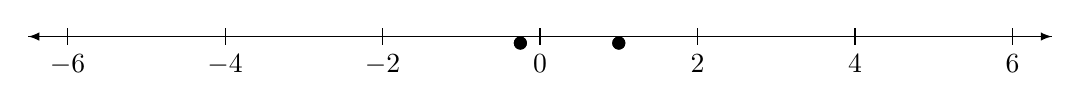
\begin{tikzpicture}
        \draw[latex-] (-6.5,0) -- (6.5,0) ;
        \draw[-latex] (-6.5,0) -- (6.5,0) ;
        \foreach \x in  {-6,-4,-2,0,2,4,6}
        \draw[shift={(\x,0)},color=black] (0pt,3pt) -- (0pt,-3pt);
        \foreach \x in {-6,-4,-2,0,2,4,6}
        \draw[shift={(\x,0)},color=black] (0pt,0pt) -- (0pt,-3pt) node[below] 
        {$\x$};
        \draw[*-o] (-0.25,0);
        \draw[*-o] (1.0,0);
       % \draw[*-o] (0.92,0) -- (2.08,0);
       % \draw[very thick    ] (0.92,0) -- (1.92,0);
        
        \end{tikzpicture}
    \end{solution}

    \vfill 
    \newpage
    \part [1] Build the chart with columns for the interval, the test
    number, evaluation at the test number, and the true/false value.

    \begin{solution}[3.25in]
    
    \begin{tabular}{|c|c|c|c|}
    \hline
     \textbf{Interval} & \textbf{Test} & $\frac{2 x + 3}{4 x +1} \leq 1$ & \textbf{True or False} \\ \hline
     $(-\infty, -1/4)$  & -1  & $-\frac{1}{3} \leq 1$ & True \\
      $(-1/4,1)$  &  0  & $3 \leq 1 $ & False \\
      $(1,\infty)$ & 2 & $\frac{7}{9} \leq 1$ & True \\ \hline
    \end{tabular}
    
    \end{solution}


    \part [1] Test each interval endpoint for inclusion or
    exclusion into the solution set.

    \begin{solution}[3.25in]
    
 \begin{tabular}{|c|c|c|}
 \hline
   \textbf{Endpoint} &  $\frac{2 x + 3}{4 x +1} \leq 1$ & \textbf{True or False} \\ \hline
    $-1/4$   & dne   & False \\
    1           & $1 \leq 1$ & True \\ \hline
 \end{tabular}
    
    \end{solution}

    \part [1] Express the solution set in either interval notation, 
    pictorially, or set builder notation.
    
    \begin{solution}
    In interval notation the solution set is $(-\infty,-\frac{1}{4}) \cup [1,\infty)$. In set builder notation,
    it is $\{x |  x < -\frac{1}{4} \mbox{ or }  x \geq  1 \}$.
    
    \end{solution}

\end{parts}


%\newpage

\question Find the vertex of each parabola.

\begin{parts}

    \part [1] $y -2 = 5(x+1)^2$.
    \begin{solution}[1.25in] The easy way is to match to $y-k = a(x-h)^2$. The match is $k=2$, $a=5$, and $h=-1$.
    The vertex is the point $(x=-1, y=2)$.    
    \end{solution}

    \part [1] $y =  3 x^2 + 2 x + 9$
    \begin{solution}[1.25in] This time we match to $y=a x^2 + b x + c$. The match is $a=3, b=2$ and $c=9$. 
    The vertex is the point 
    \begin{equation*}
      \left(x = -\frac{b}{2 a}, y = c - \frac{b^2}{4 a}\right) = (x=-\frac{1}{3}, y=\frac{26}{3}).
    \end{equation*}
    
    \end{solution}

    \part [1] $y =  x (1-x)$
    \begin{solution}[1.25in] The easy way is to remember that the x-coordinate of the vertex is the midpoint of the x-intercepts.
    The x-intercepts are 0 and 1, so the x-coordinate of the vertex is $x=1/2$. To find the y-coordinate of the vertex, paste $x=1/2$ into $y =  x (1-x)$. So the vertex is $(x=1/2, y=1/4)$.
    
    \end{solution}



\end{parts}

%\newpage

\question Morwenna grows and sells organic mustard greens. The number $q$ of
bunches of greens she can sell in a day is related to the selling
price of $p$ dollars per bunch by $q = 20 - 2 p$. 

\begin{parts}

    \part[1] Express the \emph{revenue} $R$ she gets for selling
    $q$ bunches of greens for $p$ dollars per bunch as a function
    of the selling price.

    \begin{solution}[2.25in]
    \begin{equation}
      R= p q= p ( 20 - 2 p).
    \end{equation}
    
    \end{solution}

    \part[1] Find the selling price $p$ that will maximize Morwenna's
    daily revenue.
 \begin{solution}[2.25in] The graph of revenue is a downward facing parabola with intercepts $p=0$ and $p=10$.
 To maximize the revenue, Morwenna should sell each bunch of mustard greens for $5$ dollars (the midpoint of 0 and 10).
    

    
    \end{solution}
\end{parts}

%\vfill
%\newpage

\question Sketch a pretty good graph of $y = (x-1)^2 (x+1)^2$.
\begin{solution}[3.25in]
    \includegraphics[scale=0.25]{desmos-graph(41).png}
\end{solution}

\question [1]  Given that $P$ is a third degree polynomial such that
(a) $P$ has a zero with multiplicity of 2 at 5; (b) $P$ has a zero with multiplicity 1 
at -2; and $P(0) = 1$, find an equation for $P$.

\begin{solution} Using the data about the degree, zeros and their multiplicities, the polynomial is $P(x) = a (x-5)^2 (x+2)$,
where $a$ is some number. Using  $P(0) = 1$, gives $a=1/50$. So $P(x) = \frac{1}{50} (x-5)^2 (x+2)$,

\end{solution}
\end{questions}
\end{document}
